\subsection{Oracle Adapter}

Oracle provides replication support between Oracle databases using DataGuard. Additionally, there are commercial products like GoldenGate (from Oracle) that make the change log from Oracle available to external applications. In the absence of available open-source technology to solve this problem, a company has two options. It can either license the commercial solution with the associated fees and feature availability or try to develop and support its own solution. At the time LinkedIn was evaluating change capture technologies, GoldenGate lacked required features like BLOB/CLOB support. LinkedIn has implemented an Oracle change-capture mechanism based on triggers which we describe next.

A simple approach to get the change log from Oracle is to have a timestamp column with every row. A trigger on the table updates the timestamp column with the current time on an insert or update to the row as shown in Figure~\ref{fig:Tablewithtimestamp}. The adapter then issues a query to the database to get all the changed rows.

\begin{figure}
\centering
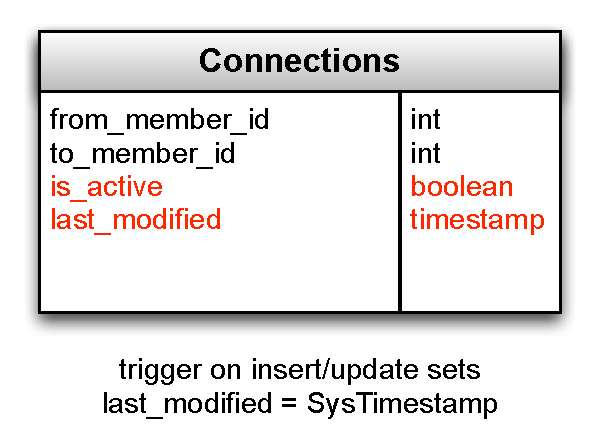
\epsfig{file=figures/timestamp-based-cdc.eps, scale=0.5}
\vspace*{-2ex}
\caption{Timestamp based CDC attempt}
\label{fig:Tablewithtimestamp}
\vspace*{-2ex}
\end{figure}

This however has a problem. Timestamps in this mechanism are set at the time of the change to the row, not at transaction commit. Long running transactions might have rows that changed long before the transaction finally commits. Thus, this query will miss changes from the database. For example in Figure~\ref{fig:tx1tx2}, tx2 commits before tx1 but t2 > t1. If the query happens between the two commits, lastTimeStamp is t2 and tx1 is missed. We can try some padding to reread rows that changed since $lastTimeStamp~-~n$ seconds but this is very error prone.

\begin{figure}
\centering
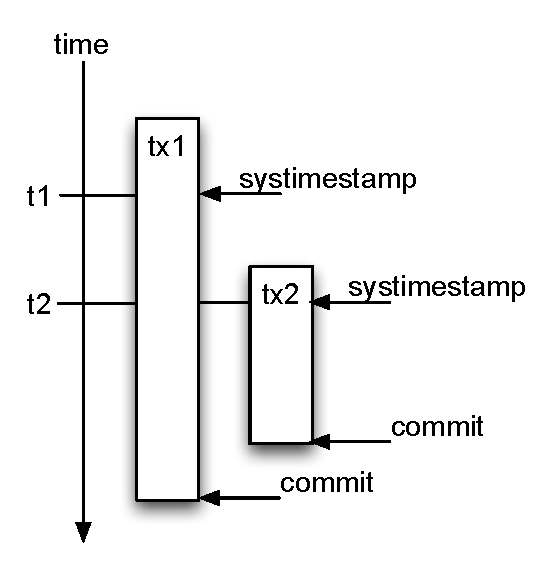
\epsfig{file=figures/timestamp-commit-reordering.eps, scale=0.50}
\vspace*{-2ex}
\caption{Timestamp based CDC: commit reordering}
\label{fig:tx1tx2}
\vspace*{-2ex}
\end{figure}
Oracle 10g and later versions provide a feature that provides the ora\_rowscn pseudo column which contains the internal Oracle clock (SCN - system change number) at transaction commit time. By default, ora\_rowscn is available at the block granularity but tables can be created with an option to provide ora\_rowscn at the row granularity. We can now query the database to fetch all rows that changed since the last rowscn but unfortunately ora\_rowscn is not an indexable column. To get around this problem, we add a regular column scn to the table and create an index on the column. The default value of scn is set to infinity. After commit, the ora\_rowscn for the affected rows is set. Every so often, we run a statement to update the scn column.

\begin{verbatim}
update T set scn = ora_rowscn
where scn = infinity;
\end{verbatim}

The query to select the changed rows since lastScn now becomes

\begin{verbatim}
select * from T 
where scn > lastScn 
AND ora_rowscn > lastScn;
\end{verbatim}

This works to get changes from a single table. However, transaction can span multiple tables in a database and these changes need to be transported to the consumer while preserving the transaction boundary. To solve this, we add a per database table TxLog that has the indexed scn column. We add a txn column to all the other tables that we wish to get changes from. We have a trigger than allocates txn from a sequence and adds an entry to the TxLog table on every transaction commit as shown in Figure~\ref{fig:txlog}. 

\begin{figure}
\centering
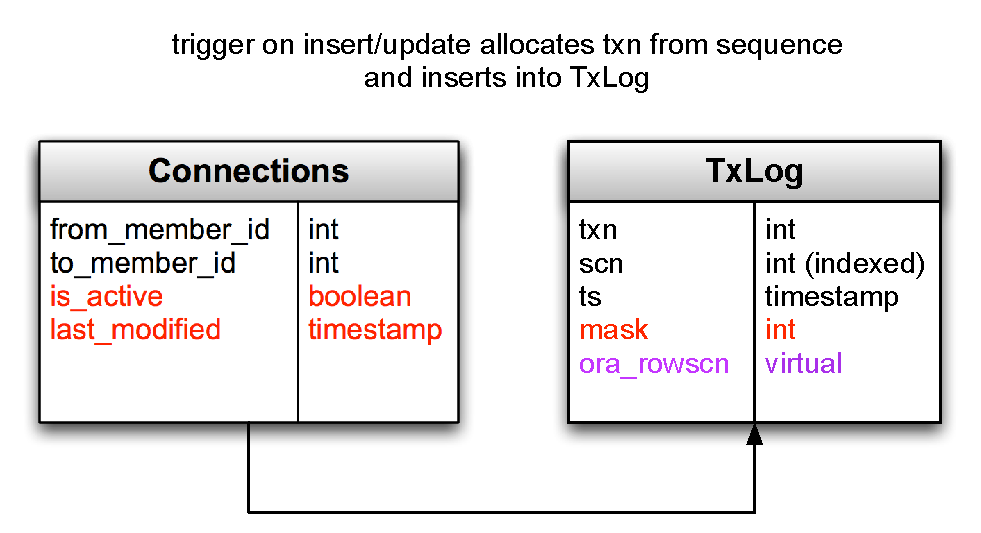
\epsfig{file=figures/txlog-based-cdc.eps, scale=0.50}
\vspace*{-2ex}
\caption{Trigger based CDC}
\label{fig:txlog}
\vspace*{-2ex}
\end{figure}

Changes can now be pulled using the following query

\begin{verbatim}
select src.* from T src, TxLog 
where scn > lastScn 
AND ora_rowscn > lastScn 
AND src.txn = TxLog.txn;
\end{verbatim}

The trigger-based approach used by the Oracle adapter has a couple of drawbacks. Firstly, it can miss intermediate changes to rows because it is only guaranteed to return the latest state of every changed row. This is not a correctness problem, but if possible, it is desirable to surface every change made to the row to the consumer.
Secondly, triggers and the associated tables that they update cause additional load in terms of reads and writes on the source database.


